\documentclass{standalone}
\usepackage{tikz}
\usetikzlibrary{calc}
\begin{document}
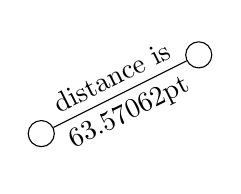
\begin{tikzpicture}

\node[draw,circle] (a) at (0,0) {};
\node[draw,circle] (b) at (2,1) {};

\draw let
    \p1 = ($(b)-(a)$),
    \n{distance} = {veclen(\y1,\x1)}
in
    (a) -- node[above,sloped]{distance is}
           node[below,sloped]{\n{distance}}
           (b) {};

\end{tikzpicture}
\end{document}
